% Generated by pysimcount.pffigure -- do not edit; regenerate instead.
% figure: B-all-by-formula -- Every formula at measured r
% source: results/np-main/seed1/results.json
% metric=t gatebase=ct merged
% seed=1 t=n template=simcount synth=pygridsynth
% git_commit=01d3c275ceae2840002bd1aaea68f59b987c4975 git_dirty=False
% source_sha256=0dd1c9775f148df550d3d3f68cfeee1d2d060b7913324535bbf1533b52b4d2c2
% derived: B-all-by-formula.tex with Lie-Trotter S1 removed by pysimcount.figdrop (Lie-Trotter S1 alone spans 42% of the original y-axis); removed legends: Lie-Trotter S1; source_sha256=d01c2c0d39d1c94c9f0805ba1bd831d3bc25b0efc0bebbe53e9e811a9e13443a
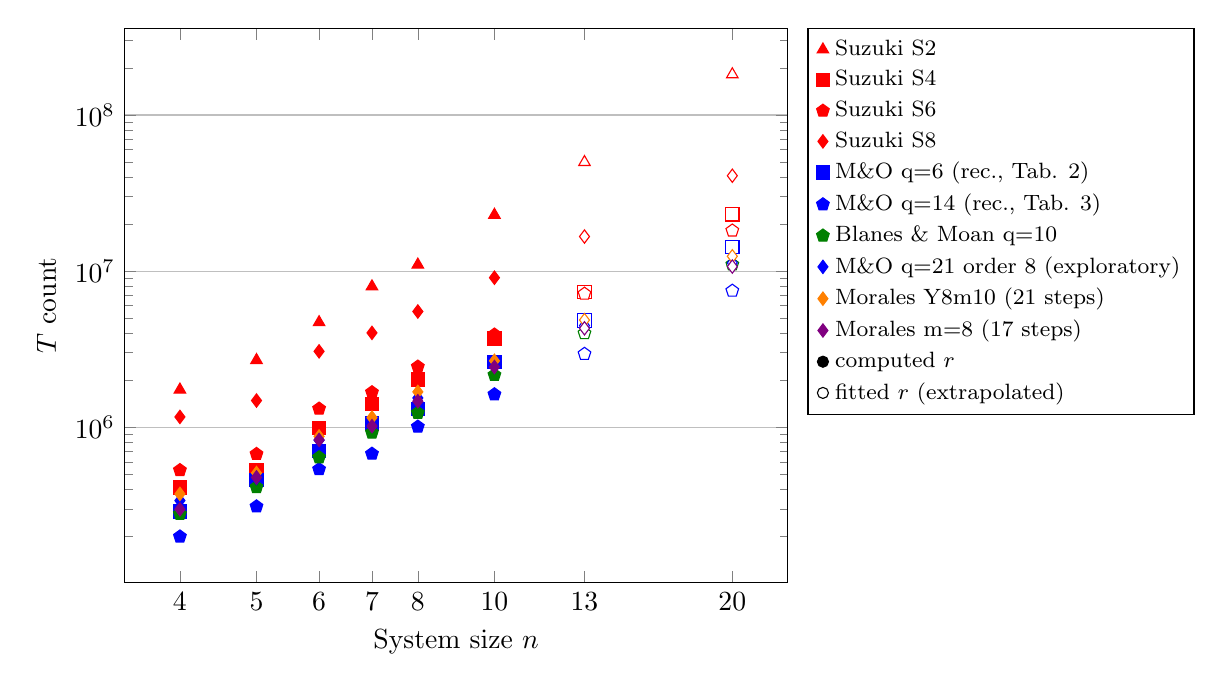
\begin{tikzpicture}
  \begin{loglogaxis}[
    width=10cm,
    xlabel={System size $n$},
    ylabel={$T$ count},
    xtick={4,5,6,7,8,10,13,20},
    xticklabels={4,5,6,7,8,10,13,20},
    ymajorgrids=true,
    legend pos=outer north east,
    legend cell align=left,
    legend style={font=\footnotesize},
  ]
    % r from power-law fit (extrapolation); one legend entry per series
    \addplot[only marks, red, mark=triangle*, mark size=2.4pt, mark options={solid, fill=red}] coordinates {
      (4,1739724)
      (5,2687776)
      (6,4698130)
      (7,7969260)
      (8,10989048)
      (10,22900530)
    };
    \addlegendentry{Suzuki S2}
    % r from power-law fit (extrapolation); one legend entry per series
    \addplot[only marks, red, mark=triangle*, mark size=2.4pt, mark options={solid, fill=white}, forget plot] coordinates {
      (13,49822284)
      (20,181860528)
    };
    \addplot[only marks, red, mark=square*, mark size=2.4pt, mark options={solid, fill=red}] coordinates {
      (4,410856)
      (5,534710)
      (6,987026)
      (7,1404340)
      (8,2020560)
      (10,3710728)
    };
    \addlegendentry{Suzuki S4}
    % r from power-law fit (extrapolation); one legend entry per series
    \addplot[only marks, red, mark=square*, mark size=2.4pt, mark options={solid, fill=white}, forget plot] coordinates {
      (13,7377150)
      (20,23100384)
    };
    \addplot[only marks, red, mark=pentagon*, mark size=2.4pt, mark options={solid, fill=red}] coordinates {
      (4,530964)
      (5,673708)
      (6,1314412)
      (7,1673760)
      (8,2443080)
      (10,3919244)
    };
    \addlegendentry{Suzuki S6}
    % r from power-law fit (extrapolation); one legend entry per series
    \addplot[only marks, red, mark=pentagon*, mark size=2.4pt, mark options={solid, fill=white}, forget plot] coordinates {
      (13,7156932)
      (20,18178252)
    };
    \addplot[only marks, red, mark=diamond*, mark size=2.4pt, mark options={solid, fill=red}] coordinates {
      (4,1164552)
      (5,1483068)
      (6,3062680)
      (7,4023074)
      (8,5513378)
      (10,9073036)
    };
    \addlegendentry{Suzuki S8}
    % r from power-law fit (extrapolation); one legend entry per series
    \addplot[only marks, red, mark=diamond*, mark size=2.4pt, mark options={solid, fill=white}, forget plot] coordinates {
      (13,16651540)
      (20,40825400)
    };
    \addplot[only marks, blue, mark=square*, mark size=2.4pt, mark options={solid, fill=blue}] coordinates {
      (4,288000)
      (5,461360)
      (6,701600)
      (7,1058148)
      (8,1310224)
      (10,2607488)
    };
    \addlegendentry{M\&O q=6 (rec., Tab. 2)}
    % r from power-law fit (extrapolation); one legend entry per series
    \addplot[only marks, blue, mark=square*, mark size=2.4pt, mark options={solid, fill=white}, forget plot] coordinates {
      (13,4833430)
      (20,14317248)
    };
    \addplot[only marks, blue, mark=pentagon*, mark size=2.4pt, mark options={solid, fill=blue}] coordinates {
      (4,199480)
      (5,310776)
      (6,538016)
      (7,676044)
      (8,1008044)
      (10,1624000)
    };
    \addlegendentry{M\&O q=14 (rec., Tab. 3)}
    % r from power-law fit (extrapolation); one legend entry per series
    \addplot[only marks, blue, mark=pentagon*, mark size=2.4pt, mark options={solid, fill=white}, forget plot] coordinates {
      (13,2948400)
      (20,7479184)
    };
    \addplot[only marks, green!50!black, mark=pentagon*, mark size=2.4pt, mark options={solid, fill=green!50!black}] coordinates {
      (4,278692)
      (5,413072)
      (6,641424)
      (7,923508)
      (8,1235364)
      (10,2161552)
    };
    \addlegendentry{Blanes \& Moan q=10}
    % r from power-law fit (extrapolation); one legend entry per series
    \addplot[only marks, green!50!black, mark=pentagon*, mark size=2.4pt, mark options={solid, fill=white}, forget plot] coordinates {
      (13,3998064)
      (20,11023104)
    };
    \addplot[only marks, blue, mark=diamond*, mark size=2.4pt, mark options={solid, fill=blue}] coordinates {
      (4,339064)
      (5,473304)
      (6,826404)
      (7,1090942)
      (8,1540862)
      (10,2478630)
    };
    \addlegendentry{M\&O q=21 order 8 (exploratory)}
    % r from power-law fit (extrapolation); one legend entry per series
    \addplot[only marks, blue, mark=diamond*, mark size=2.4pt, mark options={solid, fill=white}, forget plot] coordinates {
      (13,4477512)
      (20,11284878)
    };
    \addplot[only marks, orange, mark=diamond*, mark size=2.4pt, mark options={solid, fill=orange}] coordinates {
      (4,374088)
      (5,509288)
      (6,873540)
      (7,1153080)
      (8,1685200)
      (10,2664264)
    };
    \addlegendentry{Morales Y8m10 (21 steps)}
    % r from power-law fit (extrapolation); one legend entry per series
    \addplot[only marks, orange, mark=diamond*, mark size=2.4pt, mark options={solid, fill=white}, forget plot] coordinates {
      (13,4859064)
      (20,12445250)
    };
    \addplot[only marks, violet, mark=diamond*, mark size=2.4pt, mark options={solid, fill=violet}] coordinates {
      (4,298248)
      (5,477630)
      (6,829500)
      (7,1016752)
      (8,1467828)
      (10,2431170)
    };
    \addlegendentry{Morales m=8 (17 steps)}
    % r from power-law fit (extrapolation); one legend entry per series
    \addplot[only marks, violet, mark=diamond*, mark size=2.4pt, mark options={solid, fill=white}, forget plot] coordinates {
      (13,4303300)
      (20,10697428)
    };
    \addlegendimage{only marks, black, mark=*, mark options={fill=black}}
    \addlegendentry{computed $r$}
    \addlegendimage{only marks, black, mark=*, mark options={fill=white}}
    \addlegendentry{fitted $r$ (extrapolated)}
  \end{loglogaxis}
\end{tikzpicture}
